
%%%%%%%%%%%%%%%%%%%%%%%%%%%%%%%%%%%%%%%%%%%%%%%%%%%%%%%%%%%%%%%%%%%%%%%%%%%%%%%%%%%%%%%%%%%%%%%%%%%%%%%%%%%%
% Author: Omar Portillo
%%%%%%%%%%%%%%%%%%%%%%%%%%%%%%%%%%%%%%%%%%%%%%%%%%%%%%%%%%%%%%%%%%%%%%%%%%%%%%%%%%%%%%%%%%%%%%%%%%%%%%%%%%%%

%Abstract: 0.5
%Intro: 2
%Bg: 2
%Approach/Architecture: 3
%Experiments/Results: 5
%Related Work: 1
%Conclusions: 0.5
%References:  1

%%%%%%%%%%%%%%%%%%%%%%%%%%%%%%%%%%%%%%%%%%%%%%%%%%%%%%%%%%%%%%%%%%%%%%%%%%%%%%%%%%%%%%%%%%%%%%%%%%%%%%%%%%%%
% Defining document class + packages to be used
%%%%%%%%%%%%%%%%%%%%%%%%%%%%%%%%%%%%%%%%%%%%%%%%%%%%%%%%%%%%%%%%%%%%%%%%%%%%%%%%%%%%%%%%%%%%%%%%%%%%%%%%%%%%

\documentclass[runningheads,a4paper]{llncs}

\usepackage{amssymb}
\setcounter{tocdepth}{3}
\usepackage{graphicx}
\usepackage{epstopdf}
\usepackage[linesnumbered,ruled,vlined]{algorithm2e}

\usepackage{url}
\newcommand{\keywords}[1]{\par\addvspace\baselineskip
\noindent\keywordname\enspace\ignorespaces#1}

%Commands needed to define the max size a float can have without been presented
% ALONE in a page.
\renewcommand\topfraction{0.85}
\renewcommand\bottomfraction{0.85}
\renewcommand\textfraction{0.1}
\renewcommand\floatpagefraction{0.85}

%Commands to redice the space before and after floats (like table,fig or alg)
\setlength\floatsep{1.25\baselineskip plus 3pt minus 2pt}
\setlength\textfloatsep{1.25\baselineskip plus 3pt minus 2pt}
\setlength\intextsep{1.25\baselineskip plus 3pt minus 2 pt}

\setlength{\belowcaptionskip}{-7.5pt}
\setlength{\abovecaptionskip}{-2.5pt}

\begin{document}

%%%%%%%%%%%%%%%%%%%%%%%%%%%%%%%%%%%%%%%%%%%%%%%%%%%%%%%%%%%%%%%%%%%%%%%%%%%%%%%%%%%%%%%%%%%%%%%%%%%%%%%%%%%%
% TITLE + AUTHORS' INFORMATION
%%%%%%%%%%%%%%%%%%%%%%%%%%%%%%%%%%%%%%%%%%%%%%%%%%%%%%%%%%%%%%%%%%%%%%%%%%%%%%%%%%%%%%%%%%%%%%%%%%%%%%%%%%%%

\mainmatter  % start of an individual contribution

% first the title is needed
\title{Towards an Automated Approach to Use Expert Systems
in Java Performance Testing}

% a short form should be given in case it is too long for the running head
\titlerunning{Automated Approach to Use Expert Systems
in Java Performance Testing}

% the name(s) of the author(s) follow(s) next
%
% NB: Chinese authors should write their first names(s) in front of
% their surnames. This ensures that the names appear correctly in
% the running heads and the author index.
%
\author{A. Omar Portillo-Dominguez\inst{1}\and Miao Wang\inst{1}\and Philip
Perry\inst{1} \and\\
John Murphy\inst{1} \and Nick Mitchell\inst{2}\and Peter F. Sweeney\inst{2}\and
Erik Altman\inst{2}}

\authorrunning{A.O. Portillo-Dominguez et al.}
% (feature abused for this document to repeat the title also on left hand pages)

\urldef{\mailucdconnect}\path|andres.portillo-dominguez@ucdconnect.ie,|
\urldef{\mailucd}\path|{philip.perry,miao.wang,j.murphy}@ucd.ie,|
\urldef{\mailibm}\path|{nickm,pfs,ealtman}@us.ibm.com|

% the affiliations are given next; don't give your e-mail address
% unless you accept that it will be published
\institute{Lero - The Irish Software Engineering Research Centre, Performance\\
Engineering Laboratory, UCD School of Computer Science and Informatics,
University College Dublin, Ireland\\
\mailucdconnect\\
\mailucd\\
%\url{http://www.ucd.ie/}
\and
IBM T.J. Watson Research Center,\\
Yorktown Heights, New York, USA\\
\mailibm}%\\
%\url{http://www.ibm.com/}

\toctitle{Lecture Notes in Computer Science}
\tocauthor{Authors' Instructions}
\maketitle

%%%%%%%%%%%%%%%%%%%%%%%%%%%%%%%%%%%%%%%%%%%%%%%%%%%%%%%%%%%%%%%%%%%%%%%%%%%%%%%%%%%%%%%%%%%%%%%%%%%%%%%%%%%%
% Abstract 
%%%%%%%%%%%%%%%%%%%%%%%%%%%%%%%%%%%%%%%%%%%%%%%%%%%%%%%%%%%%%%%%%%%%%%%%%%%%%%%%%%%%%%%%%%%%%%%%%%%%%%%%%%%%
\vspace{-15pt}
\begin{abstract}
Performance testing in highly distributed environments is very challenging.
Specifically, the identification of performance issues and the diagnosis of their root causes 
are time-consuming and complex tasks which usually require multiple tools
and heavily rely on expertise. To simplify these tasks, hence increasing the
productivity and reducing the dependency on human experts, many
researchers have been developing tools with built-in expertise for non-expert users. However, managing the huge
volume of data generated by these tools in highly distributed
environments prevent their efficient usage in performance testing. To
address these limitations, this paper presents a lightweight approach to automate the usage of 
expert tools in the performance testing of Java systems. In this paper,
we use a tool named Whole-system Analysis of Idle Time to demonstrate how our research work solves this problem. The 
validation involved two experiments, using real-life applications, which
assessed the overhead of the approach and the time savings that it can bring to the
analysis of performance issues. The results proved the benefits of the approach by achieving
a significant decrease in the time invested in performance analysis while 
introducing a low overhead in the tested system.

\vspace{-3pt}
\keywords{Performance testing, automation, performance analysis, expert tools,
distributed systems}
\end{abstract}
\vspace{-22pt}
%%%%%%%%%%%%%%%%%%%%%%%%%%%%%%%%%%%%%%%%%%%%%%%%%%%%%%%%%%%%%%%%%%%%%%%%%%%%%%%%%%%%%%%%%%%%%%%%%%%%%%%%%%%%
% Introduction
%%%%%%%%%%%%%%%%%%%%%%%%%%%%%%%%%%%%%%%%%%%%%%%%%%%%%%%%%%%%%%%%%%%%%%%%%%%%%%%%%%%%%%%%%%%%%%%%%%%%%%%%%%%%
\vspace{-4pt}
\section{Introduction}
\vspace{-7pt}
It is an accepted fact in the industry that performance is a critical dimension
of quality and should be a major concern of any software project. This is
especially true at enterprise-level, where system performance plays a central
role in using the software to achieve business goals. However it is not
uncommon that performance issues occur and materialize into serious problems in a 
significant percentage of applications (i.e. outages on production environments
or even cancellation of software projects). For example, a 2007 survey applied to 
information technology executives \cite{Compuware1} reported that 50\% of them
had faced performance problems in at least 20\% of their deployed applications.

This situation is partially explained by the pervasive nature of
performance, which makes it hard to assess because performance is practically
influenced by every aspect of the design, code, and execution environment
of an application. The latest trends in information technology (such
as Service Oriented
Architecture\footnote{http://msdn.microsoft.com/en-us/library/aa480021.aspx} and 
Cloud Computing\footnote{http://csrc.nist.gov/publications/nistpubs/800-145/SP800-145.pdf}) 
have also augmented the complexity of applications further complicating activities related to
performance. 

Under these conditions, it is not surprising that doing performance
testing is complex and time-consuming. A special challenge, documented by
multiple authors \cite{Woodside2007,trevor1,Angelopoulos2012}, is that current
performance tools heavily rely on human experts to understand their
output. Also multiple sources are commonly required to diagnose performance
problems, especially in highly distributed environments. For instance in Java: thread dumps, 
garbage collection logs, heap dumps, CPU utilization and memory usage, are a few
examples of the information that a tester could need to understand the performance 
of an application. This problem increases the expertise required to do
performance analysis, which is usually held by only a small number of experts 
inside an organization\cite{Spear2009}. Therefore it could potentially lead to
bottlenecks where certain activities can only be done by these experts,
impacting the productivity of the testing teams\cite{Angelopoulos2012}.

To simplify the performance analysis and diagnosis, hence increasing the
productivity and reducing the dependency on expert knowledge, many researchers
have been developing tools with built-in expertise for non-expert
users \cite{Altman2010,pat7,Angelopoulos2012}. However, various limitations
exist in these tools that prevent their efficient usage in the performance
testing of highly distributed environments. The data collection usually needs
to be controlled manually which, in an environment composed of multiple nodes to
monitor and coordinate simultaneously, is very time-consuming and error-prone
due to the vast amount of data to collect and consolidate. This challenge is
more complex because the data needs to be processed periodically during the
test execution to get incremental results. A similar problem occurs 
with the outputs, where a tester commonly gets multiple
reports (possible one for each monitored node per data processing cycle). This
reduces the usefulness of the reports as a tester must manually
correlate their findings.

Even though these limitations might be manageable in small testing environments,
they prevent the efficient usage of these tools in bigger environments. To
exemplify this problem, let's use the Eclipse Memory Analyzer
Tool\footnote{http://www.eclipse.org/mat/} (MAT), which is a popular open source
tool to identify memory consumption issues in Java. If a tester wants to use MAT
to monitor an environment composed of 100 nodes during a 24-hour test run and 
get incremental results every hour, she would need to manually coordinate the
data gathering of memory snapshots and the generation of the tool's reports.
These steps conducted periodically for the 100 nodes every hour, which
yields a total of 2400 iterations. Moreover the tester would have to review
the multiple reports she would get per hour to evaluate if any memory issues
exist. As an alternative, she may concentrate the analysis on a single node,
assuming it is representative of the whole system. However it generates the risk of
potentially overlooking issues in the tested application.

In addition to these challenges, the overhead generated by any technique
should be low
%, and steady through time, 
to minimize the impact it has in the
tested environment (i.e. inaccurate results or abnormal behavior). Otherwise the
technique would not be suitable for performance testing. For example,
instrumentation\footnote{http://msdn.microsoft.com/en-us/library/aa983649(VS.71).aspx}
is currently a common approach used in performance analysis to gather input data
\cite{Yang1,Hangal1,Csallner1,Chen2}. However, it has the downside of obscuring
the performance of the instrumented applications, hence compromising the results of 
performance testing. Similarly, if a tool requires heavy human effort, this might limit its 
applicability. On the contrary, automation could encourage the adoption of a technique. 
As documented by the authors in \cite{Shahamiri1}, this strategy has proven
successful in performance testing.

Finally, to ensure that our research is helpful to solve real-life
problems in the software industry, we have been working with our industrial
partner, IBM System Verification Test (SVT), to understand the challenges
in their day-to-day testing activities. Their feedback confirms that there is a 
real need to simplify the usage of expert tools so that testers can do
analysis tasks in less time. Another key need of enterprise scale users is that
tests match key use cases seen by real users, and further that test teams be
able to convey their results in a meaningful way with teams in development and
in operations (the so-called “DevOps” model). The IBM Whole-system Analysis of
Idle Time tool (WAIT)\footnote{http://wait.ibm.com} used in this work meets
these needs. This publicly available expert system helps to identify the
main performance inhibitors that exist in Java systems. Moreover WAIT is
sufficiently lightweight and easy to use that it can be and has been deployed in
production, test and development environments.

This paper proposes a lightweight automation approach that addresses the common
usage limitations of an expert system in performance testing. Furthermore,
during our research development work we have successfully applied our approach
to the WAIT tool. Our work was validated through two experiments using
real-world applications. The first experiment evaluates the overhead introduced
by our approach. The second experiment assesses the productivity gains that our
approach can bring to the performance testing process. The results provided evidence 
about the benefits of the approach: It drastically reduced the effort required by a
tester to use and analyze the outputs of the selected expert tool (WAIT). This
usage simplification translated into a quicker identification of performance issues, 
including the pinpointing of the responsible classes and methods. Also the
introduced overhead was low (between 0\% to 3\% when using a common industry
\emph{Sampling Interval} of 480 seconds).

The main contributions of this paper are: 
%\\\\

1. A novel lightweight approach to automate the usage of expert systems in
performance testing of distributed Java systems.

2. A practical validation of the approach consisting of an implementation
around the WAIT tool. The validation consists of two experiments using
real-life applications. The first experiment demonstrates that the overhead of
our approach is minimal, and the second experiment demonstrates the productivity
benefit of our approach.
\\\\
The rest of this paper is structured as follows: Section \ref{Background}
discusses the background. Section \ref{ProposedApproach} explains the proposed
approach, while Section \ref{ExperimentalEvaluation} explores the experimental 
evaluation and results. Section \ref{RelatedWork} shows the related work.
Finally Section \ref{Conclusions} presents the conclusions and future work.


%%%%%%%%%%%%%%%%%%%%%%%%%%%%%%%%%%%%%%%%%%%%%%%%%%%%%%%%%%%%%%%%%%%%%%%%%%%%%%%%%%%%%%%%%%%%%%%%%%%%%%%%%%%%
% Background
%%%%%%%%%%%%%%%%%%%%%%%%%%%%%%%%%%%%%%%%%%%%%%%%%%%%%%%%%%%%%%%%%%%%%%%%%%%%%%%%%%%%%%%%%%%%%%%%%%%%%%%%%%%%
\vspace{-7pt}
\section{Background}
\label{Background}
\vspace{-7pt}
\emph{Idle-time analysis} is a methodology that is used to identify the root
causes of under-utilized resources. This approach, proposed in
\cite{Altman2010}, is based on the observed behavior that performance problems in multi-tier
applications usually manifest as idle time of waiting threads.
WAIT is an expert system that implements the idle-time analysis and identifies
the main performance inhibitors that exist on a system. Moreover it has proven successful in simplifying the detection of performance issues and their root causes in Java
systems \cite{Altman2010,Wu1}.

WAIT is based on non-intrusive sampling mechanisms available at
Operating System level (i.e. ``ps'' command in a Unix environment) and the Java
Virtual Machine (JVM), in the form of \emph{Javacores}
\footnote{http://www-01.ibm.com/support/docview.wss?uid=swg27017906\&aid=1}
(diagnostic feature to get a quick snapshot of the JVM state, offering
information such as threads, locks and memory). The fact that WAIT uses standard
data sources makes it non-disruptive, as no special flags or instrumentation are
required to use it. Another important aspect of being non-disruptive, is that
the application does not need to be restarted. This is more important when diagnosing performance
problems in production environments. Furthermore WAIT requires infrequent
samples to perform its diagnosis, so it also has low overhead.

From an end-user perspective, WAIT is simple: A user only needs to
collect as much data as desired, upload it to a public web page (wait.ibm.com)
and get a report with the findings. This process can be repeated multiple times to monitor a
system through time. Internally, WAIT uses an engine built on top of a set of 
expert rules to perform the analysis. \figurename ~\ref{fig_WAITReport} shows an
example of a WAIT Report. The top area summarizes the usage of resources (i.e.
CPU or memory) and the types of threads. The bottom section shows all
the performance inhibitors that have been identified, ranked by frequency and impact. 
Also each color indicates a different problem category. For example, in
\figurename ~\ref{fig_WAITReport} the top issue appeared in 53\% of the samples
and affected 7.6 threads on average. Moreover the affected resource was the
network and the issue was caused by waiting on the database.

\begin{figure}[!h]
\centering
\includegraphics[totalheight=.29\textheight,width=1.0\textwidth]{bigExampleReportConsolidated}
\caption{Example of WAIT Report}
\label{fig_WAITReport}
\end{figure}

Given its strengths, WAIT is a promising candidate to reduce the
dependence on a human expert and reduce the time required for performance 
analysis. However, as with many expert systems that could be used for testing 
distributed software systems, the volume of data generated can be difficult to 
manage and efficiently process this data can be an impediment to their
adoption. The effort required to manually collect data to feed WAIT and the number 
of reports a tester gets from the WAIT system are approximately linear with
respect to the number of nodes and the update frequency of the results. This makes 
WAIT a good candidate to apply our proposed approach.


%%%%%%%%%%%%%%%%%%%%%%%%%%%%%%%%%%%%%%%%%%%%%%%%%%%%%%%%%%%%%%%%%%%%%%%%%%%%%%%%%%%%%%%%%%%%%%%%%%%%%%%%%%%%
% Proposed Approach
%%%%%%%%%%%%%%%%%%%%%%%%%%%%%%%%%%%%%%%%%%%%%%%%%%%%%%%%%%%%%%%%%%%%%%%%%%%%%%%%%%%%%%%%%%%%%%%%%%%%%%%%%%%%
\vspace{-7pt}
\section{Proposed Approach and Architecture}
\label{ProposedApproach}
\vspace{-7pt}

\subsection{Proposed Approach}
\vspace{-7pt}
The objective of this work was to automate the manual processes involved
in the usage of an expert system (ES). This logic will execute concurrently with
the performance test, periodically collecting the required samples, then
incrementally processing them with the ES to get a consolidated
output. This scenario is depicted in \figurename ~\ref{fig_Overview} where the
automation shields the tester from the complexities of using the ES, so
that she only needs to interact with the load testing tool.

\vspace{-1pt}
\begin{figure}[!h]
\centering
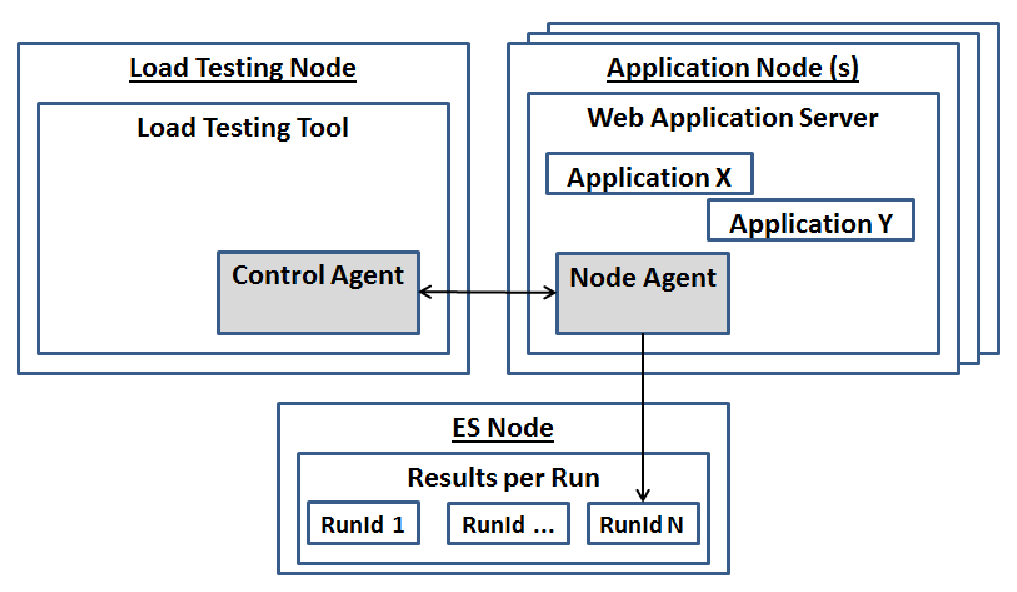
\includegraphics[totalheight=.18\textheight,width=0.8\textwidth]{architecture_dwait}
\caption{Contextual View of the Proposed Approach}
\label{fig_Overview}
\end{figure}

The detailed approach is depicted in the \figurename
~\ref{fig_ApproachDiagram}. In order to start, some inputs  are required: The list of 
nodes to be monitored; a \emph{Sampling Interval} to control how
often the samples will be collected; a \emph{Time Threshold} to define the maximum 
time between data uploads; a \emph{Hard Disk Threshold} to define the maximum
storage quota for collected data (to prevent its uncontrolled growth); and a
\emph{Backup} flag to indicate if the collected data should be backed up before any 
cleaning occurs.

%\vspace{-7pt}
%\begin{itemize}
%	\item The list of nodes to be monitored.
%	\item The \emph{Sampling Interval} to control how often the samples will be
%	collected.
%	\item The \emph{Backup} flag to indicate if the collected data should be
	% backed up before any cleaning occurs.
%	\item The \emph{Time Threshold} to define the maximum time between data
%	uploads.
%	\item The \emph{Hard Disk Threshold} to define the maximum storage quota for
%	collected data (to prevent its uncontrolled growth).
%\end{itemize}

\begin{figure}[!h]
\centering
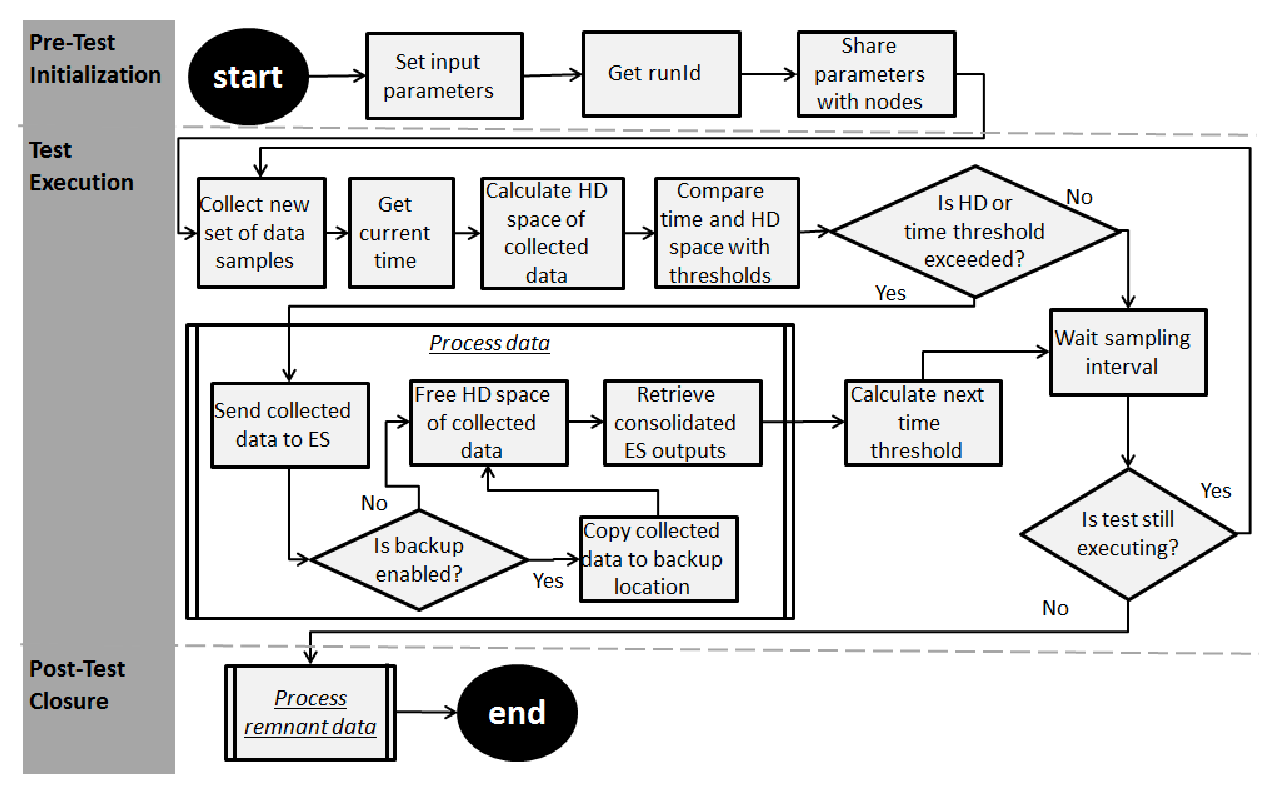
\includegraphics[totalheight=.35\textheight,width=1.0\textwidth]{ApproachDiagram}
\caption{Process Flow - Automation approach}
\label{fig_ApproachDiagram}
\end{figure}

The process starts
%, in parallel to the performance test, 
by initializing the
configured parameters. Then it gets a new \emph{RunId}, value which will
uniquely identify the test run and its collected data. This value is then
propagated to all the nodes. On each node, the \emph{Hard Disk Usage Threshold} and  
the next \emph{Time Threshold} are initialized. These
thresholds make the approach adaptable to different usage scenarios. For
example, if a tester prefers to get updated results as soon as new data is
collected, she could set the thresholds close to zero.

%Moreover it is not uncommon that
%an ES require some processing time to generate its outputs. In this scenario,
%bigger thresholds would be preferable.

Then each node starts the following loop in parallel until the performance test
finishes: A new set of data samples is collected. After the collection finishes,
the system checks if any of the two thresholds have been reached. If either of
these conditions has occurred, the data is sent to the expert system (labeling the 
data with the \emph{RunId} so that information from different nodes can be
identified as part of the same test run). If a \emph{Backup} was enabled, the data 
is copied to the backup destination before it is deleted to free space and keep
the HD usage below the threshold. As certain data collections can be costly (i.e. 
the generation of a memory dump in Java can take several minutes and require
hundreds of megabytes of HD), this step could be useful to perform further
off-line analysis of the collected data. Next updated outputs from the ES are
retrieved and the new \emph{Time Threshold} is calculated. Finally, the logic
awaits the \emph{Sampling Interval} before a new iteration starts.

Once the performance test finishes, any remaining collected data is sent (and
backed up if configured) so that it is also processed by the
expert system. Lastly the data is cleared and the final outputs of the expert system are obtained.

\vspace{-7pt}
\subsection{Architecture}
\vspace{-7pt}
The approach is implemented with the architecture
presented in \figurename ~\ref{fig_components}. It is composed of two main components:
The \emph{Control Agent} is responsible of interacting with the load
testing tool (LTT) to know when the test starts and ends. It is also responsible
of getting the runId and propagate it to all the nodes. The second component is
the \emph{Node Agent} which is responsible for the collection, upload, backup and cleanup in each node. 
On both agents the control logic and its \emph{Helper} classes (i.e. the
calculation of the thresholds in the \emph{Node Agent}), is independent of the target ES and LTT. On the contrary, the logic that interfaces with the tools need to be
customized. To minimize the code changes, this logic is encapsulated in two
\emph{Wrapper} packages which are only accessed through interfaces.
This is depicted in \figurename ~\ref{fig_wrapper} which shows the class diagram
of the package \emph{ES Wrapper}. It contains a main interface
\emph{IExpertSystem} to expose all required actions and an abstract
class for common functionality. This class hierarchy is then extended to
support a specific ES on different operating systems.

\begin{figure*}
\centering
\begin{minipage}[b]{.67\textwidth}

\centering
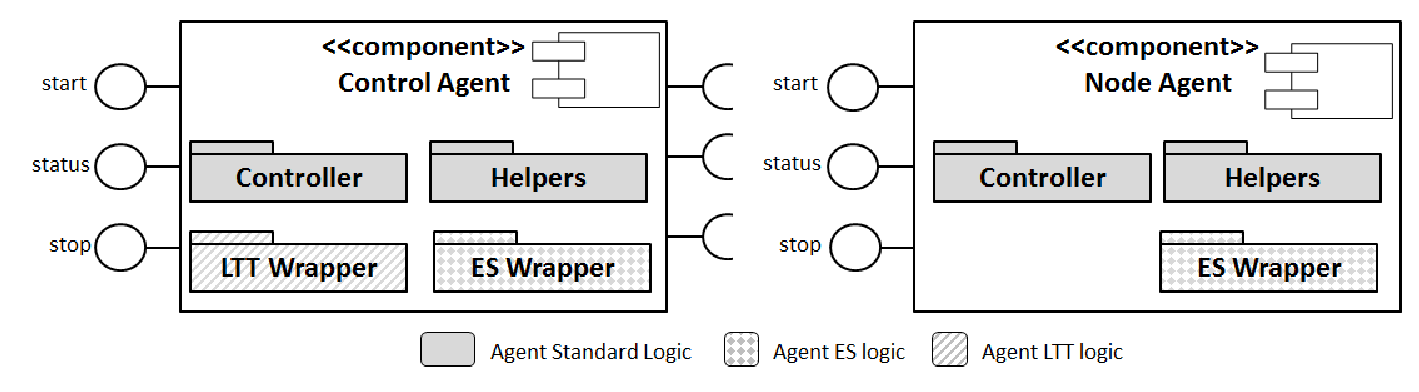
\includegraphics[totalheight=.25\textheight,width=1.0\textwidth]{Components}
\caption{Component Diagram of Architecture}
\label{fig_components}

\end{minipage}\qquad
\begin{minipage}[b]{.27\textwidth}

\centering
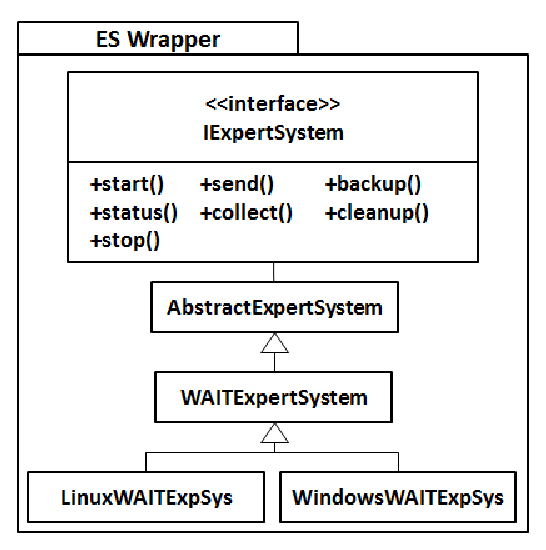
\includegraphics[totalheight=.25\textheight,width=1.0\textwidth]{Wrapper}
\caption{Class Diagram of ES Wrapper package}
\label{fig_wrapper}

\end{minipage}
\end{figure*}

These two components communicate through commands, following the
\emph{Command}\footnote{http://www.oodesign.com/command-pattern.html} Design
Pattern: The \emph{Control Agent} invokes them, while the \emph{Node Agent}
implements the logic in charge of executing each concrete command. An example of
these interactions is depicted in \figurename ~\ref{fig_SeqDiagram}. Once a
tester has started a performance test (step 1), the \emph{Control Agent}
propagates the action to all the nodes (steps 2 to 4). Then each \emph{Node
Agent} performs its periodic data collection (steps 5 to 9) until any of the
thresholds is satisfied and the data is sent to the ES (steps 10 and 11). This
continues iteratively until the test ends. At that moment, the \emph{Control Agent} 
propagates the stop action (steps 21,22 and 24). At any time, the tester might
choose to review the intermediate results of the ES (steps 12 to 14) until
getting the final results (steps 25 to 27).

%\vspace{-5pt}
\begin{figure}[!h]
\centering
\includegraphics[totalheight=.38\textheight,width=1.0\textwidth]{SequenceDiagram}
\caption{Sequence diagram of the automated approach}
\label{fig_SeqDiagram}
\end{figure}
%\vspace{-5pt}

%%%%%%%%%%%%%%%%%%%%%%%%%%%%%%%%%%%%%%%%%%%%%%%%%%%%%%%%%%%%%%%%%%%%%%%%%%%%%%%%%%%%%%%%%%%%%%%%%%%%%%%%%%%%
% Experimental Setup / Experiments
%%%%%%%%%%%%%%%%%%%%%%%%%%%%%%%%%%%%%%%%%%%%%%%%%%%%%%%%%%%%%%%%%%%%%%%%%%%%%%%%%%%%%%%%%%%%%%%%%%%%%%%%%%%%
\vspace{-7pt}
\section{Experimental Evaluation}
\label{ExperimentalEvaluation}
%\vspace{-5pt}

%In this section the developed prototype and the experimental setup are
%presented. Then the experiments are described and their results discussed.

\vspace{-7pt}
\subsection{Prototype}
\vspace{-7pt}
Based on the proposed approach, a prototype has been developed
in conjunction with our industrial partner IBM. The \emph{Control Agent} was
implemented as a plugin for the Rational Performance Tester (RPT)
\footnote{http://www-03.ibm.com/software/products/us/en/performance}, which is a
load testing tool commonly used in the industry; the \emph{Node Agent} was
implemented as a Java Web Application, and WAIT was the selected expert system
due to its analysis capabilities (discussed in Section \ref{Background}).

Once the agents are installed, WAIT can be configured as
any other resource in RPT as shown in \figurename ~\ref{fig_config}. Similarly,
during a test WAIT can be monitored in the \emph{Performance Report} of RPT
under the \emph{Resource View}. It is depicted in \figurename ~\ref{fig_mon},
which shows some metrics that a tester can check per node: The number
of monitored processes, the started data collections and the completed ones.
Additionally, the consolidated WAIT report is accessible within RPT, so a tester
does not need to leave RPT during the whole performance test. This is shown in \figurename ~\ref{fig_report}. 
%The benefits of this report will be explained in Section
% \ref{Experiment_2_Results} as part of the experimental results.

%--------------------------------------------------
\vspace{-5pt}
\begin{figure*}
\centering
\begin{minipage}[b]{.50\textwidth}

\centering
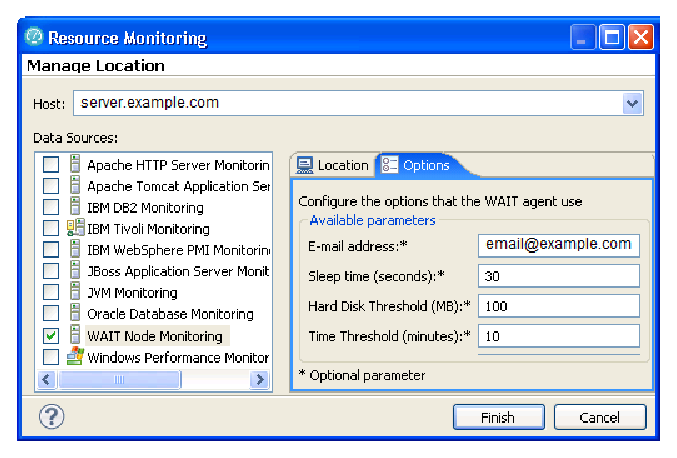
\includegraphics[totalheight=.25\textheight,width=1.0\textwidth]{WAIT-config}
\caption{WAIT configuration in RPT}
\label{fig_config}

\end{minipage}\qquad
\begin{minipage}[b]{.44\textwidth}

\centering
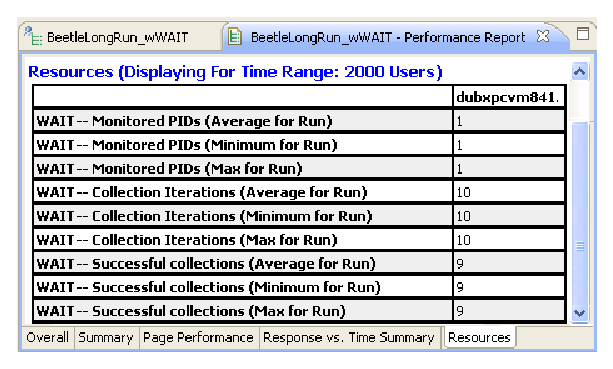
\includegraphics[totalheight=.25\textheight,width=1.0\textwidth]{WAIT-monitoring}
\caption{WAIT monitored in RPT}
\label{fig_mon}

\end{minipage}
\end{figure*}
\vspace{-5pt}

%--------------------------------------------------

\begin{figure}[!h]
\centering
\includegraphics[totalheight=.3\textheight,width=1.0\textwidth]{WAIT-report}
\caption{WAIT Report accessible within RPT}
\label{fig_report}
\end{figure}

\vspace{-7pt}
\subsection{Experimental Set-up}
\vspace{-7pt}
Two experiments were performed. The first one aimed to evaluate if the overhead
introduced by the proposed approach was low so that it does not compromise the
results of a performance test. Meanwhile, the second experiment shows the
productivity benefits that a tester can gain by using the proposed approach.
Additionally two environment configurations were used, as shown in \figurename
~\ref{fig_env}. One was composed of an RPT node, one application node and a
\emph{WAIT Server} node; the other was composed of a RPT node, a load balancer node, 
two application nodes and a \emph{WAIT Server} node. All connected by a 10-GBit
LAN.

\vspace{-1pt}
\begin{figure}[!h]
\centering
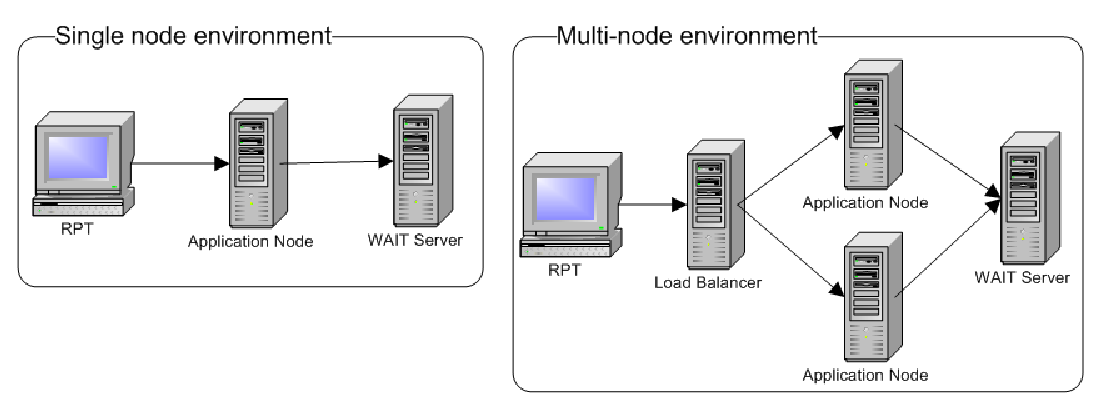
\includegraphics[totalheight=.14\textheight,width=0.9\textwidth]{Environments}
\caption{Environment Configurations}
\label{fig_env}
\end{figure}

The RPT node ran over Windows XP with an Intel Xeon CPU at
2.67 GHz and 3GB of RAM using RPT 8.2.1.3. The \emph{WAIT Server} was run over
Red Hat Enterprise Linux Server 5.9, with an Intel Xeon CPU at 2.66 GHz and 2GB of
RAM using Apache Web Server 2.2.3. Each application node was a 64-bit Windows
Server 2008, with an Intel Xeon E7-8860 CPU at 2.26 GHz and 4GB of RAM
running Java 1.6.0 IBM J9 VM (build 2.6). Finally, the load balancer node had
the same characteristics of the \emph{WAIT Server} node. 

\vspace{-7pt}
\subsection{Experiment \#1: Overhead Evaluation}
\vspace{-7pt}

The objective here was to quantify the overhead of the proposed approach and
involved the assessment of four metrics: Throughput (hits per second), response
time (milliseconds), CPU (\%) and memory (MB) utilization. All metrics were
collected through RPT. Furthermore, two real-world applications were used:
iBatis JPetStore 4.0 \footnote{http://sourceforge.net/projects/ibatisjpetstore/}
which is an upgraded version of Sun's Pet Store, an e-commerce shopping cart. It
ran over an Apache Tomcat 6.0.35. The other application was IBM WebSphere Portal 
8.0.1 \footnote{http://www-03.ibm.com/software/products/us/en/portalserver},
a leading solution in the enterprise portal market. It ran over an IBM WebSphere
Application Server 8.0.0.5.

%\vspace{-7pt}
%\begin{itemize}
%	\item The applications alone to get a baseline.
%	\item The applications with manual WAIT data collection.
%	\item The applications with an automated WAIT.
%\end{itemize}

Firstly, the overhead was measured in a single-node environment using three
combinations of WAIT: The applications alone to get a baseline, the applications
with manual WAIT data collection, and the applications with an automated
WAIT. For each combination using WAIT, the \emph{Sampling Interval} was
configured to 480 seconds (a commonly used value) and 30 seconds (minimum value 
recommended for WAIT). The remaining test configurations were suggested by IBM SVT to
reflect real-world conditions: A workload of 2,000 concurrent users; a duration
of 1 hour; a \emph{Hard Disk Threshold} of 100MB; and a \emph{Time Threshold} of
10 minutes. Finally, each combination was repeated three times.

For JPetStore, each test run produced around 500,000 transactions. The results
presented in \tablename ~\ref{PetStore1} showed that using WAIT with a
\emph{Sampling Interval} of 480 seconds had practically no impact in terms of
response time and throughput. Furthermore the difference in resource consumption
between the two modalities of WAIT was around 1\%.  This difference was
mostly related to the presence of the \emph{Node Agent} because the uploaded
data was very small (around 200KB every 10 minutes). When a
\emph{Sampling Interval} of 30 seconds was used, the impact on response time
and throughput appeared. Since the throughput was similar between the WAIT
modalities, the impact was caused by the \emph{Javacore} generation as it is
the only step shared between the modalities. On average, the generation of a
\emph{Javacore} took around 1 second. Even though this cost was insignificant in
the higher \emph{Sampling Interval}, with 30 seconds the impact was visible.
Additionally the difference in response times between the two modalities of WAIT
was caused by the upload and backup processes (around 4MB of data every 10
minutes), as the cost of the \emph{Node Agent} presence had been previously
measured. In terms of resource consumption, the differences between the WAIT
modalities remained within 1\%.

\vspace{-5pt}
\begin{table}[!h]
\caption{JPetStore - Overhead Results}
\label{PetStore1}
\centering
\begin{tabular}{p{0.2\textwidth}|p{0.16\textwidth}|p{0.16\textwidth}|p{0.15\textwidth}|p{0.13\textwidth}|p{0.16\textwidth}}
\hline
\bfseries WAIT Modality & \bfseries Avg Response Time (ms)& \bfseries Max
Response Time (ms)& \bfseries Avg Throughput (hps)& \bfseries Avg CPU Usage
(\%) & \bfseries Avg Memory Usage (MB)\\
\hline
None (\emph{Baseline}) 	& 1889.6	& 44704.0	& 158.8 	& 36.9 		& 1429\\
Manual, 480s 			& 0.0\% 	& 0.0\%		& 0.0\%		& 1.1\% 	& 3.0\%\\
Automated, 480s 		& 0.0\%		& 0.0\%		& 0.0\% 	& 2.0\% 	& 3.7\%\\
Manual, 30s 			& 1.6\%		& 0.4\%		& -3.1\% 	& 1.47\% 	& 4.1\%\\
Automated, 30s 			& 4.4\%		& 0.5\%		& -4.0\% 	& 2.53\% 	& 4.4\%\\
\hline
\end{tabular}
\end{table}
\vspace{-5pt}

For Portal, each test run produced around 400,000 transactions and the
results are presented in \tablename ~\ref{Portal1}. They show similar trends
to the results in \tablename ~\ref{PetStore1}, but a few
key differences were identified: First, the impact on response time and
throughput were visible even with the \emph{Sampling Interval} of 480 seconds.
Also, the differences between the results for the two \emph{Sampling Interval}
were bigger. As the experimental conditions were the same, it was initially
assumed that these differences were related to the dissimilar functionality of the 
tested applications. This was confirmed after analyzing the \emph{Javacores} generated 
by Portal, which allowed the differences in behavior of Portal to be quantified:
The average size of a \emph{Javacore} was 5.5MB (450\% bigger than JPetStore's), its 
average generation time was 2 sec (100\% bigger than JPetStore's), with a maximum 
generation time of 3 sec (100\% bigger than JPetStore's).

%\vspace{-5pt}
\begin{table}[!h]
\caption{Portal - Overhead Results}
\label{Portal1}
\centering
\begin{tabular}{p{0.2\textwidth}|p{0.16\textwidth}|p{0.16\textwidth}|p{0.15\textwidth}|p{0.13\textwidth}|p{0.16\textwidth}}
\hline
\bfseries WAIT Modality & \bfseries Avg Response Time (ms)& \bfseries Max
Response Time (ms)& \bfseries Avg Throughput (hps)& \bfseries Avg CPU Usage
(\%) & \bfseries Avg Memory Usage (MB)\\
\hline
None (\emph{Baseline}) 	& 4704.75	& 40435.50	& 98.05 	& 76.73 	& 3171.20\\
Manual, 480s 			& 0.7\% 	& 0.6\%		& -0.1\%	& 0.63\% 	& 2.2\%\\
Automated, 480s 		& 3.4\%		& 1.0\%		& -2.8\% 	& 1.13\% 	& 4.1\%\\
Manual, 30s 			& 14.9\%	& 5.4\%		& -5.6\% 	& 2.23\% 	& 5.3\%\\
Automated, 30s 			& 16.8\%	& 9.1\%		& -5.7\% 	& 2.97\% 	& 6.0\%\\
\hline
\end{tabular}
\end{table}
%\vspace{-5pt}

[To explore the small differences between the runs and the potential
environmental variations that were experienced during the experiments, a Paired
t-Test
\footnote{http://www.aspfree.com/c/a/braindump/comparing-data-sets-using-statistical-analysis-in-excel/}
 was done (using a significance level of p\textless0.05) to evaluate if the
differences in response time and throughput were statistically significant.
This analysis indicated that the only significant differences existed in the
 average response time and the average throughput when using a \emph{Sampling Interval} of 30 seconds.
This analysis reinforced the conclusion that the overhead was low and the
observation that the \emph{Sampling Interval} of 480 seconds was preferable.]

A second test was done to validate that the overhead remained low in a
multi-node environment over a longer test run. This test used JPetStore and the
automated WAIT tool with a \emph{Sampling Interval} of 480 seconds. The rest of
the set-up was identical to the previous tests except the workload which was doubled
to compensate for the additional application node and the test duration which
was increased to 24 hours. Even though the results were slightly different than the
single-node run, they proved that the solution was reliable, as using the
automated approach had minimal impact in terms of response time (0.5\% 
average and 0.2\% max) and throughput (1.4\%). Moreover the consumption
of resources behaved similarly to the single-node test (an increment of 0.85\%
in CPU and 2.3\% in Memory). 

%A paired t-Test also indicated that the differences
%in response time and throughput between the runs were not significant.

In conclusion, the results of this experiment proved that the
overhead caused by the automated approach was low, therefore the results of a
performance test are not compromised. Due to the impact that the \emph{Sampling
Interval} and the application behavior could have on the overhead, it is important to 
consider these factors in the configuration. In our case, a \emph{Sampling
Interval} of 480 seconds proved efficient in terms of overhead for the two tested applications using WAIT.

\vspace{-7pt}
\subsection{Experiment \#2: Assessment of productivity benefits}
\label{Experiment_2_Results}
\vspace{-7pt}

Here the objective was to assess the benefits our approach brings to a
performance tester. First, the source code of JPetStore was modified and three
common performance issues were injected: A lock contention bug, composed of a
very heavy calculation within a synchronized block of code; an I/O latency bug,
composed of a very expensive file reading method; and a deadlock bug, composed
of an implementation of the classic ``friends bowing'' deadlock
example\footnote{http://docs.oracle.com/javase/tutorial/essential/concurrency/deadlock.html}.

%\vspace{-7pt}
%\begin{itemize}
%	\item A lock contention bug, composed of a very heavy calculation within a
%	synchronized block of code.
%	\item An I/O latency bug, composed of a very expensive file reading method.
%	\item A deadlock bug, composed of an implementation of the classic ``friends
%	bowing'' deadlock
% example\footnote{http://docs.oracle.com/javase/tutorial/essential/concurrency/deadlock.html}.
%\end{itemize}

% Is it worth put ``that much emphasys'' on this (or is it enough the previous
% approach of indicating that the same configuration was used).
Then an automated WAIT, with a \emph{Sampling Interval} of 480 seconds,
monitored the application to assess how well it was able to identify the
injected bugs and estimate the corresponding time savings in performance
analysis. All set-up parameters were identical to the multi-node test previously 
described except the duration which was one hour. Due to space
constraints, only the most relevant sections of the WAIT reports are presented.

The 1st ranked issue was not an injected bug but one related to the
clustering set-up of Tomcat.
%Surprisingly the 1st ranked issue was none of the injected bugs but a method
%named ``McastServiceImpl.receive'' which appeared in practically all the
%samples. Further analysis determined this method call was benign and related
%to the clustering functionality of Tomcat.
The 2nd ranked issue was the lock
contention. It is worth noting that both issues were
detected since the early versions of the report from the tool and their
high frequency (above 96\% of the samples) could have led a tester to pass this
information to the development team so that the diagnosis could start far ahead
of the test completion. The final report reinforced the presence of these issues 
by offering similar rankings. \figurename ~\ref{fig_run1_bugs12}.a shows the
results of the early report, while ~\ref{fig_run1_bugs12}.b shows the results of 
the final report.

\begin{figure}[!h]
\centering
\includegraphics[totalheight=.25\textheight,width=1\textwidth]{big_issues12_run1_earlyVsFinalReport}
\caption{Top detected performance issues in modified JPetStore application}
\label{fig_run1_bugs12}
\end{figure}

\begin{figure}[!h]
\centering
\includegraphics[totalheight=.25\textheight,width=1\textwidth]{lockContentionIssue_WAITvsEclipse_Highlighted}
\caption{Lock contention issue in the WAIT report and the actual source code}
\label{fig_issue2_vs_code}
\end{figure}

After identifying an issue, a tester can see more details, including the type of
problem, involved class, method and method line. \figurename
~\ref{fig_issue2_vs_code} shows the information of our Lock Contention bug,
which was located in the class LockContentionBug, the method generateBug and the
line 20. When comparing this information with the actual code, one can see it
is precisely the line where the bug was injected (taking a class lock before
doing a very CPU intensive logic). In 3rd place the report showed a symptom of
the lock contention issue, suggesting it was a major problem (the issues were
correlated by comparing their information, which pinpointed to the same class and
method). Finally, the I/O latency bug was identified in 4th place. \figurename
~\ref{fig_issues34} shows the details of these issues.

\begin{figure}[!h]
\centering
\includegraphics[totalheight=.25\textheight,width=1\textwidth]{big_issue3and4_run1_finalReportDetailsMerge}
\caption{Details of issues ranked 3rd and 4th}
\label{fig_issues34}
\end{figure}

The deadlock issue did not appear in this test run, somehow prevented by the
lock contention bug which had a bigger impact than planned. As in any regular
test phase, the identified bugs were fixed and a new run was done to review
if any remaining performance issues existed. Not surprisingly, the deadlock bug
appeared. \figurename ~\ref{fig_dlissue_vs_code} shows the information of our
Deadlock bug, which was located in the line 30 of the DeadLockBug class. This is
precisely the line where the bug was injected (as the deadlock occurs when the
friends bow back to each other).
%\vspace{-5pt}
\begin{figure}[!h]
\centering
\includegraphics[totalheight=.23\textheight,width=1\textwidth]{deadlockIssue_DetailsVsEclipse_Highlight}
\caption{Deadlock issue in the WAIT report and the actual source code}
\label{fig_dlissue_vs_code}
\end{figure}
%\vspace{-5pt}

%Is it worth adding it . . . let's see ``space" after applying the other
% feedback:
%It further corroborated that the introduced overhead was low. ???

As all injected bugs were identified, including the involved classes and
methods, this experiment was considered successful. In terms of time, two main
savings were documented. First, the automated approach practically reduced the
effort of using WAIT to zero. After a one-time installation which took no more
than 15 minutes for all nodes, the only additional effort required to use the
automated approach were a few seconds spent configuring it (i.e. to change the
\emph{Sampling Interval}). The second time saving occurred in the analysis of the 
WAIT reports. Previously, a tester would have ended with multiple reports. Now a 
tester only needs to monitor a single report which is refreshed periodically.

Overcoming the usage constraints of WAIT also allowed to exploit
WAIT's expert knowledge capabilities. Even though it might be hard to define an
average time spent identifying performance issues, a conservative estimate of
2 hours per bug could help to quantify these savings. In our experiment,
instead of spending an estimated 6 hours analyzing the issues, it was
possible to identify them and their root causes in a matter of minutes with the 
information provided by the WAIT report. As seen in the experiment, additional
time can be saved if the relevant issues are reported to developers in parallel to
the test execution. This is especially valuable in long-term runs which
are common in performance testing and typically last several days.

To summarize these experimental results, they were very promising because it
was possible to measure the productivity benefits that a tester can gain by using
WAIT through our proposed automation approach: After a quick installation
(around 5 minutes per node), the time required to use the automated WAIT was
minimal. Moreover a tester now only needs to monitor a single WAIT report, which
offers a consolidated view of the results. A direct consequence of these
time savings is the reduction in the dependence on human expert knowledge and
a reduced effort required by a tester to identify performance issues, hence
improving the productivity.

\vspace{-7pt}
\subsection{Threats to Validity}
\vspace{-7pt}
Like any empirical work, there are some threats to the validity of these
experiments. First the possible environmental noise that could affect the test
environments because they are not isolated. To mitigate this, multiple runs were
executed for each identified combination. Another threat was the selection of
the tested applications. Despite being real-world applications, their limited
number implies that not all types of applications have been tested and wider
experiments are needed to get more general conclusions. However, there is no
reason to believe that the presented approach is not applicable to other
environments.

%%%%%%%%%%%%%%%%%%%%%%%%%%%%%%%%%%%%%%%%%%%%%%%%%%%%%%%%%%%%%%%%%%%%%%%%%%%%%%%%%%%%%%%%%%%%%%%%%%%%%%%%%%%%
% Related Work
%%%%%%%%%%%%%%%%%%%%%%%%%%%%%%%%%%%%%%%%%%%%%%%%%%%%%%%%%%%%%%%%%%%%%%%%%%%%%%%%%%%%%%%%%%%%%%%%%%%%%%%%%%%%

%\pagebreak

\vspace{-7pt}
\section{Related Work}
\label{RelatedWork}
\vspace{-7pt}
%Avritzer2,Avritzer3,
The idea of applying automation in the performance testing domain is not new.
However, most of the research has focused on automating the generation of load
test
suites\cite{Elvira1,Bayan1,Zhang1,Briand1,Chen1,Garousi1,Xingen1}.
For example \cite{Bayan1} proposes an approach to automate the generation of test 
cases based on specified levels of load and combinations of resources.
Similarly, \cite{Chen1} presents an automation framework that separates the
application logic from the performance testing scripts to increase the
reusability of the test scripts. Meanwhile \cite{Xingen1} presents a framework
designed to automate the performance testing of web applications
and which internally utilizes two usage models to simulate the users’ behaviors
more realistically.

Regarding performance analysis, a high percentage of the proposed
techniques require some type of instrumentation. For example, the authors in
\cite{Yang1} instrument the source code of the monitored applications to mine
the sequences of call graphs under normal operation, information which is
later used to infer any relevant error patterns. A similar case occurs with
the works presented in \cite{Hangal1,Csallner1} which rely on instrumentation to dynamically 
infer invariants within the applications and detect programming errors; or the
approach proposed by \cite{Chen2} which uses instrumentation to capture execution paths to determine
the distributions of normal paths and look for any significant deviations in
order to detect errors. In all these cases, the instrumentation would obscure
the performance of an application during performance testing hence discouraging
their usage. On the contrary, our proposed approach does not require any
instrumentation.

Moreover the authors of \cite{Jiang2009} present a non-intrusive approach which
automatically analyzes the execution logs of a load test to identify performance
problems. As this approach only relies on load testing results, it can not
determine root causes. A similar approach is presented in \cite{Malik1} which
aims to offer information about the causes behind the issues. However it can
only provide the subsystem responsible of the performance deviation. On the
contrary, our approach allows the applicability of the idle-time analysis in the
performance testing domain through automation, which allows the identification
of the classes and methods responsible for the performance issues. Moreover the
techniques presented in \cite{Jiang2009,Malik1} require information from previous runs 
to baseline their analysis, information which might not always be available.

Finally, the authors of \cite{mon3,Barham1} present frameworks to
monitor software services. Both monitor the resource utilization and the
component interactions within a system, but target different technologies
(\cite{mon3} focuses on Java and \cite{Barham1} on Microsoft technologies).
Unlike these works, which have been designed to assist on operational support activities, 
our proposed approach has been designed to address the specific needs of a tester in the 
performance testing, isolating her from the complexities of an expert system.

%%%%%%%%%%%%%%%%%%%%%%%%%%%%%%%%%%%%%%%%%%%%%%%%%%%%%%%%%%%%%%%%%%%%%%%%%%%%%%%%%%%%%%%%%%%%%%%%%%%%%%%%%%%%
% Section 7: Conclusions
%%%%%%%%%%%%%%%%%%%%%%%%%%%%%%%%%%%%%%%%%%%%%%%%%%%%%%%%%%%%%%%%%%%%%%%%%%%%%%%%%%%%%%%%%%%%%%%%%%%%%%%%%%%%
\vspace{-7pt}
\section{Conclusions and Future Work}
\label{Conclusions}
\vspace{-7pt}

The identification of performance problems in highly
distributed environments is complex and time-consuming. Even though
researchers have been developing expert systems to simplify this task, various
limitations exist in those tools that prevent their effective usage in
performance testing. To address these limitations, this work proposed a novel
approach to automate the usage of an expert system in a distributed testing
environment. A prototype was developed around the WAIT tool and then its
benefits and overhead were assessed. The results showed that the introduced overhead was low 
(between 0\% to 3\% when using a common industry \emph{Sampling Interval}). Also
the results showed the time savings gained by applying the approach. In our case, the effort
to utilize WAIT in distributed environments was reduced to seconds. This optimization then simplified the identification of
performance issues. In our case, all defects injected in JPetStore were detected in a matter of minutes
using WAIT's consolidated outputs. In contrast, a manual analysis might have
taken hours. Thus, the approach was shown to have a low overhead and to reduce
the time required to analyze performance issues, thereby reducing the costs
associated with performance testing. 


Future work will focus on assessing the approach and its benefits through
broader experiments with our industrial partner IBM with a special interest in 
the trade-off between the \emph{Sampling Interval} and the nature of the
applications. It will also be investigated how best to exploit the functional 
information that can be obtained from a test environment to improve the
idle-time analysis.

%%%%%%%%%%%%%%%%%%%%%%%%%%%%%%%%%%%%%%%%%%%%%%%%%%%%%%%%%%%%%%%%%%%%%%%%%%%%%%%%%%%%%%%%%%%%%%%%%%%%%%%%%%%%
% Section 8: Acknowledgements
%%%%%%%%%%%%%%%%%%%%%%%%%%%%%%%%%%%%%%%%%%%%%%%%%%%%%%%%%%%%%%%%%%%%%%%%%%%%%%%%%%%%%%%%%%%%%%%%%%%%%%%%%%%%
\vspace{-8pt}
\section*{Acknowledgments}
\vspace{-7pt}
We would like to thanks Amarendra Darisa and Patrick O'Sullivan, from IBM SVT,
as their experience in performance testing helped us through the scope
definition and validation. This work was supported, in part, by Science
Foundation Ireland grant 10/CE/I1855 to Lero - the Irish Software Engineering
Research Centre (www.lero.ie).

\vspace{-8pt}
% Between 12 - 24 \ldots 18 sounds like a good number!
\bibliographystyle{splncs}
\bibliography{dwait_manual,dwait}

%\section*{Appendix: Figures Printing Test}

\end{document}


\cite{Gartner2008}
